\subsection{1. Stufe - Strukturelle �bereinstimmung}
Wie in \cite{hummel08} wird in der ersten Stufe der Suche versucht die angebotenen Interfaces herauszusuchen, die strukturell mit dem erwarteten Interface �bereinstimmen. Zu diesem Zweck wird ein Structural-Type-Matcher verwendet, der in Abschnitt \ref{structTypeMatcher} beschrieben wird. Dar�ber hinaus werden weitere Type-Matcher verwendet (siehe Abschnitte \refs{exactTypeMatcher}{wrapperTypeMatcher}), die das Matching zweier Typen auf der Basis der Beziehung, in der diese beiden Typen zueinander stehen, feststellen. Allgemein beschrieben, kann durch jeden dieser Type-Matcher festgestellt werden, ob sich ein Typ in einen anderen Typ konvertieren l�sst.\\\\
Die Konvertierung erfolgt zur Laufzeit �ber die Erzeugung von Proxies, die ihre Methodenaufrufe delegieren. So wird bspw. bei der Konvertierung eines Objektes von TypA in ein Objekt von TypB ein Proxy-Objekt f�r TypB erzeugt, welches die Methodenaufrufe auf dem Objekt von TypA delegiert (vgl. \abbref{combinated_components}).\\\\
Hummel hatte hierzu bereits auf einige Matcher von Zaremski und Wing \cite{moormann} zur�ckgegriffen, die in dieser Arbeit ebenfalls zum Einsatz kommen (siehe Abschnitte \refs{exactTypeMatcher}{specTypeMatcher}). Weiterhin wurde in \cite{hummel08} ein Anwendungsfall f�r einen Matcher skizziert, der in der Lage ist Container-Typen zu ihren enthaltenen Typen zu matchen. Auf diese Idee wird in den Abschnitten \ref{wrappedTypeMatcher} und \ref{wrapperTypeMatcher} weiter eingegangen. Die Definitionen der Matcher beziehen sich vorrangig auf die Programmiersprache Java, weshalb grundlegend von einer nominalen Typkonformit�t auszugehen ist.\\\\
Die Typen seien in einer Bibliothek $\text{L}$ in folgender Form zusammengefasst:
\begin{table}[H]
\centering
\begin{tabular}{|p{6cm}|p{10cm}|}
\hline
\hline
\centering\textbf{Regel} & \textbf{Erl�uterung} \\
\hline
\hline
$L ::= TD\text{*}$ & Eine Bibliothek \emph{L} besteht aus einer Menge von Typdefinitionen.\\
\hline
$TD ::= PD | RD$ & Eine Typdefinition kann entweder die Definition eines provided Typen (PD) oder eines required Typen (RD) sein.\\
\hline
$PD ::=$ provided T extends T' $\{ FD\text{*} MD\text{*}\}$& Die Definition eines provided Typen besteht aus dem Namen des Typen \emph{T}, dem Namen des Super-Typs \emph{T'} von \emph{T} sowie mehreren Feld- und Methodendeklarationen.\\
\hline
$RD ::=$ required T $\{MD\text{*}\}$ & Die Definition eines required Typen besteht aus dem Namen des Typen \emph{T} sowie mehreren Methodendeklarationen.\\
\hline
$FD ::=$ f : T & Eine Felddeklaration besteht aus dem Namen des Feldes \emph{f} und dem Namen seines Typs \emph{T}.\\
\hline
$MD ::=$ m(T):T' & Eine Methodendeklaration besteht aus dem Namen der Methode \emph{m}, dem Namen des Parameter-Typs \emph{T} und dem Namen des R�ckgabe-Typs \emph{T'}.\\
\hline
\hline
\end{tabular}
\caption{Grammatik f�r die Definition einer Bibliothek von Typen}
 \label{tab:eIShort}
\end{table}
\noindent
Weiterhin sei die Relation $<$ auf Typen durch folgenden Regel definiert:
\begin{eqnarray*}
T < T' := \text{provided \emph{T} extends \emph{T'}} \in L \vee (\text{provided \emph{T} extends \emph{T''}} \in L \wedge T'' < T') 
\end{eqnarray*}
Dar�ber hinaus seien folgende Funktionen definiert:
\begin{gather*}
felder(T) :=  \left\{ 
				\begin{array}{l|l}
					f : T' & \text{ \emph{f : T'} ist Felddeklaration von \emph{T}}
				\end{array}
              \right\}\\
methoden(T) := \left\{ 
				\begin{array}{l|l}
					m(T'):T'' & \text{ \emph{m(T'):T''} ist Methodendeklaration von 										\emph{T}}
				\end{array}
              \right\}\\
vererbteMethoden(T,T') := \left\{
                \begin{array}{l|l}
                	  		&	T<T' \wedge m(P):R\in methoden(T) \wedge \\
					m(P):R 	& 	\exists m(P'):R'\in methoden(T').\\
							&	(P<=P') \wedge (R>=R') 
                \end{array}
              \right\}
\end{gather*}
\noindent
Das Matching eines Typs $A$ zu einem Typ $B$ wird durch die asymmetrische Relation $\matchTyp{A}{}{B}$ beschrieben. Dabei wird $A$ auch als \emph{Source-Typ} und $B$ als \emph{Target-Typ} bezeichnet.\\\\
Ein Proxy beschreibt die Konvertierung einer Menge von Target-Typen $P = \{T_1, ..., T_n\}$ in einen Proxy-Typen $X$. Die Definition eines Proxies hat dabei folgende Form:
\begin{table}[H]
\centering
\begin{tabular}{|p{6cm}|p{8cm}|}
\hline
\hline
\centering\textbf{Regel} & \textbf{Erl�uterung} \\
\hline
\hline
$PROXY ::=$\newline proxy X for PR $\{TARGET\text{*}\}$ & Eine Proxy-Definition besteht aus dem Namen des Proxy-Typs \emph{X}, dem Namen des Typs \emph{PR} f�r den der Proxy erzeugt wird. \emph{PR} kann dabei der Name eines \emph{required Interfaces} oder der eines \emph{provides Interfaces sein}. Weiterhin besteht ein Proxy aus einer Mengen von Targets, die die Basis f�r den Proxy bilden. \\
\hline
$TARGET ::=$\newline T target $\{MDEL\text{*} AZ\text{*}\}$ & Die Definition einer Targets besteht aus dem Namen des Target-Typs \emph{T}, dem Namen einer Variablen \emph{target} zur Referenzierung des Target-Objektes, sowie einer Menge aus Methodendelegationen und Attributzuweisungen.\\
\hline
$AZ ::=$ f = $TR$& Eine Attributzuweisung besteht aus dem Namen des Attributfeldes des Proxies \emph{f} und einer Targetreferenz.\\
\hline
$MDEL ::= CALLM \rightarrow DELT $  & Eine Methodendelegation besteht aus einer Methode, die auf dem Proxy aufgerufen wird (CALLM) und einem Delegationsziel (DELT), an das der Aufruf delegiert wird.\\
\hline
$CALLM ::=$\newline $m(P) : TYPECONV $  & Eine aufgerufene Methode besteht aus ihrem Namen \emph{m}, dem Namen des Parametertyps \emph{P} und einem Konverter f�r den R�ckgabetyp. \\
\hline
$DELT ::=$\newline $TR.n(TYPECONV) : R $  & Ein Delegationsziel besteht aus einer Referenz auf das Delegationsobjekt (TR), dem Methodennamen \emph{n} der am Delegationsobjekt aufzurufenden Methoden, sowie einem Konverter Parametertyp und dem Namen des R�ckgabetype \emph{R} der Methode \emph{n}.\\
\hline
$TYPECONV ::= PROXY | T$  & Ein Konverter ist entweder wiederum ein Proxy, oder ein Typ T, sofern keine Konvertierung vorgenommen wird.\\
\hline
$TR ::=$\newline $target | target.f $ & Eine Targetreferenz ist entweder die Variable f�r das Target-Objekt (\emph{target}) oder ein Feld mit dem Namen \emph{f} des Target.Objektes.\\
\hline
\hline
\end{tabular}
\caption{Grammatik f�r die Definition eines Proxies}
 \label{tab:eIShort}
\end{table}
\noindent
Zus�tzlich seien folgenden Funktionen definiert:
\begin{gather*}
targets(X) := \left\{ 
				\begin{array}{l|l}
					T 	& \text{\emph{T} ist der Name des Typs einer}\\
						& \text{Targets von \emph{X}}
				\end{array}
              \right\}\\       
delegationen(X,T) := \left\{
                \begin{array}{l|l}
m(SP):SR & m(SP):SR \rightarrow target.n(TP):TR\\
\rightarrow	& \text{ist eine Methodendelegation eines }\\
					target.n(TP):TR & \text{Targets \emph{T} mit } T \in targets(X) 
                \end{array}
              \right\}\\
zuweisungen(X,T) := \left\{
                \begin{array}{l|l}
                	f = V 	& 	f = V\text{ ist eine Attributzuweisung eines} \\
                	& \text{Targets \emph{T} mit } T \in targets(X)\\
				\end{array}
              \right\}
\end{gather*}
\subsubsection{StructuralTypeMatcher}\label{structTypeMatcher}
Ein Ziel dieser Arbeit ist es Typen, die keinerlei Assoziationen zueinander habe, miteinander zu matchen und so zu konvertieren, dass darauf aufbauend die erwartete Semantik �berpr�fen werden kann. Hierf�r soll wie auch in \cite{hummel08} die strukturelle �bereinstimmung der beiden Typen genutzt werden. Diesem Zweck dient der StructuralTypeMatcher.
\myparagraph{Szenario}
Um die grundlegenden Eigenschaften des StructuralTypeMatchers darzustellen, wird von einem Szenario ausgegangen, in dem zwei \emph{provided Interfaces} in Kombination ein \emph{required Interface} erf�llen. Dabei wird von einer Bibliothek $L$ ausgegangen, die zum einen eine Erweiterung der Typen aus dem JDK um die in \lstref{struct_scerantio_bib} definierten Typen darstellt.
\begin{figure}[H]

\begin{minipage}[b]{.4\linewidth}

\begin{lstlisting}
provided Fire extends Object{}
\end{lstlisting}

\begin{lstlisting}
provided FireState extends Object{
	isActive : boolean
}
\end{lstlisting}

 \begin{lstlisting}
provided Medicine extends Object{
	String getDescription()
}
\end{lstlisting}

\begin{lstlisting}
provided Injured extends Object{
	void heal(Medicine med)	
}
\end{lstlisting}



\end{minipage}%
\hspace{.04\linewidth}% Abstand zwischen Bilder
\begin{minipage}[b]{.56\linewidth}
\begin{lstlisting}
provided Patient extends Injured{}
\end{lstlisting}
\begin{lstlisting}
provided FireFighter extends Object{
	FireState extinguishFire(Fire fire)
}
\end{lstlisting}

\begin{lstlisting}
provided Doctor extends Object{	
	void heal( Patient pat, Medicine med )
}
\end{lstlisting}



\begin{lstlisting}
provided MedCabinet extends Object{
	med : Medicine
}
\end{lstlisting}
\end{minipage}
\begin{center}
\begin{lstlisting}[caption={Bibliothek von Typen},captionpos=b]
required MedicalFireFigther {
	void heal( Injured injured, MedCabinet med )
	boolean extinguishFire( Fire fire )	
}
\end{lstlisting}
\end{center}
\end{figure}
\noindent
Durch den StructuralTypeMatcher soll zum einen ein Matching der Form $\matchTyp{IntubatingFireFighter}{}{FireFighter}$ und $\matchTyp{IntubatingFireFighter}{}{Doctor}$ ermittelt werden. Dar�ber hinaus soll die Kombination aus $FireFighter$ und $Doctor$ in den Typ $IntubatingFireFither$ konvertiert werden. Ein Proxy $PTF$ der aus der Konvertierung der Typen $FireFighter$ und $Doctor$ in den Typ $IntubatingFireFighter$ ist in \lstref{struct_proxy} beschrieben.
\begin{lstlisting}
proxy PTF for MedicalFireFither{
	FireFighter fireFighter {
		extinguishFire(Fire):proxy PFireState for FireState{
			boolean target{
				isActive = target		
			}
		} --> fireFighter.extinguishFire(Fire):boolean
	}
		
	Doctor doctor {
		heal(Injured, MedCabinet):void--> doctor.heal(
			proxy PPatient for Patient{
				Injured injured{
					heal():void --> injured.heal():void			
				}		
			}, proxy PMedicine for Medicine{
				MedCabinet cab{
					getDescription():String --> cab.med.getDescription():String			
				}			
			}):void		
	}
}
\end{lstlisting}
%\abbref{methodDelegation_IntubatingFireFighter} zeigt, wie die Delegation der Aufrufe der Methoden des Typs $IntubatingFireFighter$ durch die o.g. Proxy-Definition erfolgen.\\\\
Dabei wird beim Aufruf der Methoden \emph{extinguishFire(Fire)} an die Methoden \emph{extinguishFire(Fire)} des Typs $FireFighter$ delegiert. Dabei wird der Parameter vom Typ $Fire$ einfach weitergereicht, ohne dass eine Konvertierung des Parameters ist in diesem Fall nicht notwendig, da der Parameter-Typ der aufgerufenen Methode und der Methode, an die der Aufruf delegiert wird, identisch sind. Dasselbe gilt f�r die R�ckgabewerte der beiden Methoden.\\\\
Der Aufruf der Methode \emph{intubate(Injured)} wird an die Methode \emph{intubate(Patient)} des Typs $Doctor$ delegiert. Dabei erfolgt eine weitere Konvertierung des Typs $Injured$ in den Typ $Patient$.

\myparagraph{Definition}
Das strukturelle Matching zwischen einem \emph{required Interface} $R$ und einem \emph{provided Interface} $P$ ist gegeben, sofern eine Methode aus $R$ zu einer Methode aus $P$ gematcht werden kann. Die Menge der aus $R$ in $P$ gematchten Methoden wird wie folgt beschrieben:
\begin{gather*}
structM(R,P) := \left\{ 
				\begin{array}{l|l}
					m(T):T' \in methoden(R)	& \exists n(S):S' \in methoden(P) .\\													&  \matchTyp{S}{egsc}{T} \wedge \matchTyp{T'}{egsc}{S'}
				\end{array}
              \right\}
\end{gather*}
Da die Notation es nicht hergibt, ist zus�tzlich zu erw�hnen, dass die Reihenfolge der Parameter in $m$ und $n$ irrelevant ist.\\\\
Die Relation $\Rrightarrow_{egsc}$ wird durch die �brigen Matcher in folgender Form beschrieben:
\begin{gather*}
\frac{\splitfrac{\matchTyp{A}{exact}{B} \wedge \matchTyp{A}{spec}{B} 
\wedge \matchTyp{A}{gen}{B}}{\wedge \matchTyp{A}{container}{B} \wedge \matchTyp{A}{content}{B}}}{\matchTyp{A}{egsc}{B}}
\end{gather*}
Das strukturelle Matching von $R$ und $P$ wird dann durch folgende Regel beschrieben. 
\begin{matcherEquivDef}{StructuralTypeMatcher}
\frac{structM(R,P) \neq \emptyset}{\matchTyp{R}{struct}{P}}
\end{matcherEquivDef}
F�r die Verwendung von $R$ muss jedoch sichergestellt werden, dass alle darin enthaltenen Methoden durch ein oder mehrere \emph{required Interfaces} innerhalb der gesamten Bibliothek $L$ gematcht werden. Folgende Funktion beschreibt daher eine Menge von \emph{provided Interfaces}, die in Kombination zu allen Methoden von $R$ eine �bereinstimmende Methode enthalten.
\begin{gather*}
cover(R,L) := \left\{ 
				\begin{array}{l|l}
					\{P_1,...,P_n\}	& P_1 \in L \wedge \text{...} \wedge P_n \in L \wedge \\
									& structM(R,P_1) \cup \text{...} \cup structM(R, P_n) = methoden(R)
				\end{array}
              \right\}
\end{gather*}
F�r $R$ kann die Exploration abgebrochen werden, wenn $cover(R,L) = \emptyset$ gilt.\\\\
Die Menge aller Konvertierungsm�glichkeiten einer Menge von \emph{provided Interfaces} $P = \{P_1,...,P_n\}$ in ein \emph{required Interface} $R$ �ber den StrucutralTypeMatcher wird durch die Funktion $Proxy_{struct}(R,P)$ beschrieben. Dazu sei $singleMDEL(X, MDEL)$ f�r einen Proxy $X$ und eine Methodendelegation $MDEL$ durch folgende Regel beschrieben.

\begin{gather*}
\frac{\splitfrac{\forall T \in targets(X).[\exists MDEL \rightarrow N \in delegationen(X,T) \wedge}{ \forall T' \in targets(X).(MDEL \rightarrow N) \not\in delegationen(X,T') \vee T' = T]}}{singleMDEL(X, MDEL)}
\end{gather*}



\begin{matcherConvDef}{StructuralTypeMatcher}{
Die Menge von Proxies, die eine Konvertierung einer Menge von \emph{provided Interfaces} $P = \{P_1,...,P_n\}$ in ein \emph{required Interface} $R$ beschreiben, wird durch die folgenden Funktion definiert:}
Proxy_{struct}(R,P) := \left\{ 
				\begin{array}{l|l}
		& \forall T \in targets(X).[zuweisungen(R,T) = \emptyset \wedge T \in P \wedge \\
		& \forall (m(SP):SR \rightarrow target.n(TP):TR) \in delegationen(X,T).[ \\
	X	& SR \in Proxy_{esgc}(SR,TR) \wedge TP \in Proxy_{esgc}(TP,SP)\\
		& \wedge m(SP):SR \in methoden(R) \wedge n(TP):TR \in methoden(T) \\
		& \wedge singleMDEL(X, m(SP):SR)]]
				\end{array}
              \right\}
\end{matcherConvDef}\\
F�r einen Proxy $X \in Proxy_{esgc}(A,B)$ gilt:
\begin{gather*}
Proxy_{esgc}(A,B) = \begin{array}{l}Proxy_{exact}(A,B) \cup Proxy_{spec}(A,B) \cup Proxy_{gen}(A,B)\\
 \cup Proxy_{container}(A,B) \cup Proxy_{content}(A,B)
 \end{array}
\end{gather*}

\subsubsection{ExactTypeMatcher}\label{exactTypeMatcher}
\myparagraph{Szenario}
Dieser Matcher stellt das Matching zweier identischer Typen fest. Das Matching kann erfolgt somit auf nominaler Ebene erfolgen.
\myparagraph{Definition}
\begin{matcherEquivDef}{ExactTypeMatcher}
\frac{}{\matchTyp{T}{exact}{T}}
\end{matcherEquivDef}
\begin{matcherConvDef}{ExactTypeMatcher}{
Eine Konvertierung eines Typs $T$ in denselben Typ ist praktisch nicht notwendig. Daher gilt:}
Proxy_{exact}(T,T) = \{T\}
\end{matcherConvDef}

\subsubsection{GenTypeMatcher}\label{genTypeMatcher}
\myparagraph{Szenario}
Dieser Matcher stellt das Matching zwischen zwei Typen her, die in einer Vererbungsbeziehung stehen. Speziell erlaubt dieser Matcher das Matching eines Supertyps als \emph{Source-Typ} mit einem Subtyp als \emph{Target-Typ}. Ausgehend von den Typen aus \lstref{example_library} wird f�r dieses Szenario auf die Typen $Injured$ als Supertyp und $Patient$ als Subtyp zur�ckgegriffen. Der GenTypeMatcher soll in diesem Fall ein Matching der Form $\matchTyp{Injured}{gen}{Patient}$ festellen. In \abbref{} ist schematisch dargestellt, wie eine Methode, die auf dem Supertyp $Injured$ aufgerufen wird, an eine Methode des Subtyps $Patient$ delegiert wird. Eine solche Delegation wird aufgrund der Regeln f�r die Methoden-Deklarationen innerhalb von Sub- und Supertypen ohne Zuhilfenahme eines Proxies erreicht.\footnote{Die Parameter-Typen m�ssen Kovarianz und die R�ckgabe-Typen Kontravarianz aufweisen. Folglich ist eine Delegation wie in \abbref{} aufgrund des Substitutionsprinzips m�glich.}
Daher muss keine Konvertierung des \emph{Target-Typs} in den \emph{Source-Typ} erfolgen. Vielmehr kann der \emph{Target-Typ} �berall dort eingesetzt werden, wo der \emph{Super-Typ erwartet wird.}
\myparagraph{Definition}
\begin{matcherEquivDef}{GenTypeMatcher}
\frac{B < A}{\matchTyp{A}{gen}{B}}
\end{matcherEquivDef}
\begin{matcherConvDef}{GenTypeMatcher}{
F�r zwei Typen $A$ und $B$ f�r die $\matchTyp{A}{gen}{B}$ gilt, ist keine Konvertierung von $B$ in $A$ notwendig. Somit gilt:}
Proxy_{gen}(A,B) = \{B\}
\end{matcherConvDef}
\subsubsection{SpecTypeMatcher}\label{specTypeMatcher}
\myparagraph{Szenario}
Analog zum GenTypeMatcher stellt der SpecTypeMatcher ebenfalls das Matching zwischen Typen fest, die in einer Vererbungsbeziehung stehen. Allerdings soll durch diesen Matcher der umgekehrte Fall abgebildet werden.
Demnach soll ausgehend von den Typen $Injured$ als Supertyp und $Patient$ als Subtyp aus \lstref{example_library}  ein Matching der Form $\matchTyp{AccidentVictim}{spec}{Injured}$ ermittelt werden. Eine Verwendung des Typen $Injured$ anstelle von $Patient$ ist nicht ohne Konvertierung m�glich. Daher als Resultat der Konvertierung �ber diesen Matcher ein Proxytyp $PPatient$ erwartet, der \lstref{} entnommen werden kann.
\begin{lstlisting}
proxy PPatient extends Patient{
	Injured injured {
		heal():void --> injured.heal():void	
	}		
}		
\end{lstlisting}
Bei genauerer Betrachtung des \emph{provided Interfaces} $Patient$ und $Injured$ f�llt auf, dass der Subtyp $Patient$ eine eigenen Methode deklariert. Bei einer Konvertierung kann diese Methode nicht delegiert werden. Der Aufruf w�rde dementsprechend fehlschlagen.\footnote{Downcast}
In \abbref{} und \abbref{} sind die Methodenaufrufe der beiden angebotenen Methoden des Typs $PPatient$ mit ihrer Delegation bzw. Fehlschlag aufgef�hrt. 
\myparagraph{Definition}
\begin{matcherEquivDef}{SpecTypeMatcher}
\frac{\inhTyp{A}{B}}{\matchTyp{A}{spec}{B}}
\end{matcherEquivDef}
\begin{matcherConvDef}{SpecTypeMatcher}{
F�r zwei Typen $A$ und $B$ f�r die $\matchTyp{A}{spec}{B}$ ist die Menge an m�glichen Proxytypen wie folgt definiert:}
Proxy_{spec}(A,B) := \left\{ 
				\begin{array}{l|l}
  & targets(X) = \{B\} \wedge zuweisungen(X,B) = \emptyset \wedge \\
X & \forall m(P):R \in vererbteMethoden(A,B).\\						  & \exists m(P):R \rightarrow target.m(P):R \in delegationen(X,B)
				\end{array}
              \right\}
\end{matcherConvDef}
\subsubsection{ContentTypeMatcher}\label{contentTypeMatcher}
\myparagraph{Szenario}
In \ref{Hum8}

%Die bisherigen Type-Matcher sind in der Lage das Matching f�r zwei Typen festzustellen, ohne daf�r R�cksicht auf deren innere Struktur nehmen zu m�ssen. Dies ist f�r identische oder hierarchisch organisierte Typen auch nicht notwendig. Es ist jedoch auch denkbar, dass sich beiden Typen auf anderem Wegen assoziieren lassen. Ein Beispiel daf�r w�re Boxed- bzw. - noch allgemeiner gefasst - Wrapper-Typen. In \abbref{cd_subclass_subwrapper} sind zwei Klassen dargestellt, die in einer solchen Beziehung zueinander stehen. Bez�glich des Matchings sind auch hier wiederum zwei F�lle zu unterscheiden. Der erste Fall, in dem das Matching des Source-Typen SubClass mit dem Typen eines Attributs wrapped des Traget-Typen SubWrapper festgestellt werden kann, ist in \abbref{sd_wrapped_sub2subwrapped} dargestellt.
%\begin{figure}[H]
%\begin{minipage}[b]{.33\linewidth}
%  \centering
%  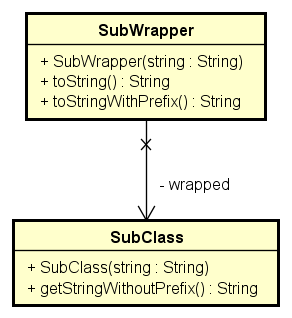
\includegraphics[width=\linewidth]{cd_subclass_subwrapper}
%  \caption{Beziehung zwischen SubClass und SubWrapper}
%  \label{abb:cd_subclass_subwrapper}

%\end{minipage}%
%\hspace{.04\linewidth}% Abstand zwischen Bilder
%\begin{minipage}[b]{.63\linewidth}


%  \centering
%  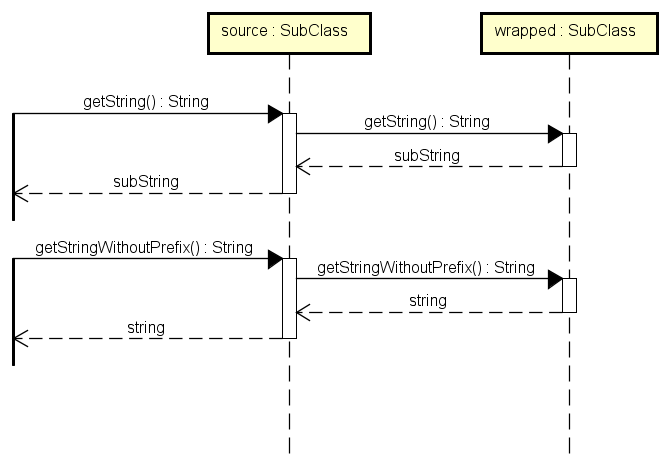
\includegraphics[width=\linewidth]{sd_wrapped_sub2subwrapped}
%  \caption{Szenario WrappedTypeMatcher}
%  \label{abb:sd_wrapped_sub2subwrapped}

%\end{minipage}
%\end{figure}
%\noindent
%Der WrappedTypeMatcher stellt das Matching f�r ein solches Szenario fest. Das Matching der beiden Typen beruht letztendlich auf einem Matching zwischen dem Source-Type und dem Typen eines Attributs des Target-Typs. Der Matcher, �ber den dieses Matching innerhalb des WrappedTypeMatchers festgestellt wird, wird als interner Matcher bezeichnet. In dem Szenario aus \abbref{sd_wrapped_sub2subwrapped} wird als interner Matcher der bereits beschriebene ExactTypeMatcher verwendet, weil der Source-Type und der Typ des Attributs wrapped identisch sind.
\myparagraph{Definition}
\begin{matcherEquivDef}{ContentTypeMatcher}
\frac{\exists f:T' \in felder(B).\matchTyp{A}{esg}{B}}{\matchTyp{A}{content}{B}}
\end{matcherEquivDef}\\
Die Relation $\Rrightarrow_{esg}$ wird durch die drei zuvor definierten Matcher beschrieben:
\begin{gather*}
\frac{\matchTyp{A}{exact}{B} \vee \matchTyp{A}{spec}{B} \vee \matchTyp{A}{gen}{B}}{\matchTyp{A}{esg}{B}}
\end{gather*}
\begin{matcherConvDef}{WrappedTypeMatcher}{
F�r zwei Typen $A$ und $B$ f�r die $\matchTyp{A}{content}{B}$ ist die Menge an m�glichen Proxytypen wie folgt definiert:}
Proxy_{content}(A,B) := \left\{ 
				\begin{array}{l|l}
  & targets(X) = \{B\} \wedge zuweisung(X,B) = \emptyset \wedge \\
X & \forall m(SP):SR \rightarrow target.f.n(TP):TR \in delegationen(X,B).\\				
  &	f \in felder(B) \wedge SR \in Proxy_{esg}(SR,TR) \wedge TP \in Proxy_{esg}(TP,SP)\\		\end{array}
              \right\}
\end{matcherConvDef}

\subsubsection{ContainerTypeMatcher}\label{containerTypeMatcher}
\myparagraph{Szenario}
%Dieser Matcher stellt das Pendant zum WrappedTypeMatcher dar. Der Unterschied bzgl. des Szenarios besteht darin, dass nun der Source-Typ derjenige ist, der ein Attribut enth�lt, f�r dessen Typ ein Matching zum Target-Typen �ber den ExactTypeMatcher, den GenTypeMatcher oder den SpecTypeMatcher festgestellt werden kann. F�r das Szenario ist wiederum von den Typen aus \abbref{cd_subclass_subwrapper} auszugehen. Die Delegation der m�glichen Methodenaufrufe am Source-Typen, sind in \abbref{sd_wrapper_subwrapped2sub} abgebildet. Hierbei ist hervorzuheben, dass zur Laufzeit das Objekt vom Target-Typen in das Attribut des Objektes vom Source-Typen injiziert wird. Dies soll in \abbref{sd_wrapper_subwrapped2sub} durch die Bezeichnung des Targets mit wrapped (dem Namen des Attributs) und target dargestellt werden. Eine Methoden-Delegation findet nur dann statt, wenn sie auch im Wrapper-Typen (Source-Typen) implementiert wurde\footnote{Implementierung von SubWrapper: siehe \appref{matcherExamples} \lstref{LST_subwrapper_impl}}.
%\myScalableFigure[0.8\linewidth]{sd_wrapper_subwrapped2sub}{Szenario WrapperTypeMatcher}{sd_wrapper_subwrapped2sub}
%\myparagraph{Definition}
\begin{matcherEquivDef}{WrapperTypeMatcher}
\frac{\exists f:T' \in felder(A).\matchTyp{T'}{esg}{B}}{\matchTyp{A}{container}{B}}
\end{matcherEquivDef}\\
\begin{matcherConvDef}{WrappedTypeMatcher}{
F�r zwei Typen $A$ und $B$ f�r die $\matchTyp{A}{container}{B}$ ist die Menge an m�glichen Proxytypen wie folgt definiert:}
Proxy_{content}(A,B) := \left\{ 
				\begin{array}{l|l}
  & targets(X) = \{B\} \wedge delegationen(X,B) = \emptyset \wedge\\
X &   \forall f=T \in zuweisung(X,B). \\
  & \exists f:T' \in felder(A). T \in Proxy_{esg}(T',B)					
				\end{array}
              \right\}
\end{matcherConvDef}\\
Ein Beispiel f�r die Verwendung des Matchers in Bezug auf das o.g. Szenario ist in \appref{wrapperMatcherExample} zu finden. Au�erdem sind dort auch weitere Szenarien aufgef�ht, in denen der GenTypeMatcher oder der SpecTypeMatcher als interner Matcher zur Anwendung kommen.



%\subsubsection{Notation zur Beschreibung der Matcher}
Die �bereinstimmung bzw. das Matching zweier Typen $ A $ und $ B $ �ber einen Matcher $ M $ wird in dieser Arbeit mit $\matchTyp{A}{M}{B}$ notiert. Weiterhin wird die Identit�t zweier Typen mit $ A = B $ beschrieben. Eine Vererbungshierarchie, in der $ A $ von $ B $ erbt, wird mit $\inhTyp{A}{B}$ beschrieben. Au�erdem ist die Adressierung der Typen von Attributen, die innerhalb eines Typs verwendet werden, notwendig. F�r die Adressierung des Typs eines Attributs $ a $ im Typ $ A $ wird $\selTyp{A}{a}$ geschrieben. Die logische Verkn�pfung der einzelnen Elemente der Sprache �ber die Quantoren und Junktoren der Pr�dikatenlogik 1. Stufe ist ebenfalls m�glich.\\\\
Die Konvertierung eines Typs $ A $ in einen Typ $ B $ wird, wie bereits erw�hnt, auf technischer Ebene �ber Proxies umgesetzt. Von daher kann die Beschreibung des Konvertierungsverfahrens eines Matchers auf die Beschreibung der Delegation einzelner Methoden beschr�nkt werden. Hierf�r wird folgende Notation verwendet:\\\\
Eine Methode $m$ enth�lt einen R�ckgabetyp $ RT $ und eine Menge von Parametertypen $ PT $. Die Menge der Parametertypen wird zur besseren Lesbarkeit auf einen Parametertyp beschr�nkt. Der Aufruf einer Methode $ m $ eines Typs $ A $ mit dem R�ckgabetyp $ RT $ und dem Parametertyp $ PT $ wird mit $ A.m( PT ) : RT $ notiert. Sofern die Konvertierung keinen Einfluss auf den R�ckgabetyp oder die Parametertypen hat, wird dies verk�rzt mit $ A.m $ beschrieben.\\\\
Die Delegation von Methodenaufrufen eines Typs wird mit dem Operator $\Rightarrow$ beschrieben. F�r eine Delegation des Aufrufs einer Methode $ m $ des Typs $ A $, welcher an einen Typ $ B $ und dessen Methode $ n $ delegiert wird, schreibt man $\delegate{A.m}{B.n}$. Ferner ist hierbei zwischen einem Source- und einem Target-Typ zu unterscheiden. Der Source-Typ befindet sich links vom Operator ($\Rightarrow$). Auf diesem Typ findet der Methodenaufruf statt. Der Target-Typ befindet sich auf der rechten Seite des Operators ($\Rightarrow$). Dieser stellt das Ziel der Delegation dar. Da bei der Delegation mitunter weitere (interne) Matcher zur Anwendung kommen m�ssen, wird hierf�r ebenfalls eine Notation ben�tigt. Daher soll die Konvertierung eines Typs $ A $ in einen Typ $B$ wird mit $\applyMatcher{B}{A}$ beschrieben. Als Voraussetzung f�r diese Konvertierung muss $\matchTyp{A}{M}{B}$ gelten.\\\\
Die folgenden Matcher werden jeweils durch ein Szenario motiviert. In den dazugeh�rigen Diagrammen ist das Object des Source-Typs (Source-Objekt) jeweils mit \emph{source} und das Objekt des Target-Typs (Target-Objekt) jeweils mit \emph{target} bezeichnet. Um die Verwendung der Implementierungen der einzelnen Matcher in Verbindung mit diesem Szenario nachvollziehen zu k�nnen, wird jeweils auf einen Abschnitt aus Anhang \ref{matcherExamples} verweisen. Dort sind Code-Beispiele f�r die Verwendung der Matcher in Bezug auf das jeweilige Szenario mit entsprechenden Nachbedingungen hinterlegt.\\\\
Die Definitionen der Matcher bestehen jeweils aus zwei Teilen. Der erste Teil (�bereinstimmung) definiert, unter welchen Bedingungen �ber den entsprechenden Matcher zwei Typen als �bereinstimmend gelten. Der zweite Teil (Konvertierung) beschreibt, wie die Delegation der Aufrufe von Methoden, die vom Source-Typ spezifiziert werden, an die Methoden, die vom Target-Typ spezifiziert werden.

\subsubsection{ExactTypeMatcher}\label{exactTypeMatcher}
\myparagraph{Szenario}
Dieser Matcher stellt das Matching zweier identischer Typen fest. In dem Szenario wird von zwei Objekten vom Typ SuperClass ausgegangen. Die Klasse SuperClass ist in \abbref{cd_superclass} dargestellt. Der Aufruf einer Methode auf dem Source-Objekt f�hrt zu einer Delgation der Methode an das Target-Objekt (siehe \abbref{sd_exact_super}).
\begin{figure}[H]
\begin{minipage}[b]{.33\linewidth}
  \centering
  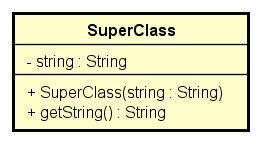
\includegraphics[width=\linewidth]{cd_superclass}
  \caption{SuperClass}
  \label{abb:cd_superclass}

\end{minipage}%
\hspace{.04\linewidth}% Abstand zwischen Bilder
\begin{minipage}[b]{.63\linewidth}


  \centering
  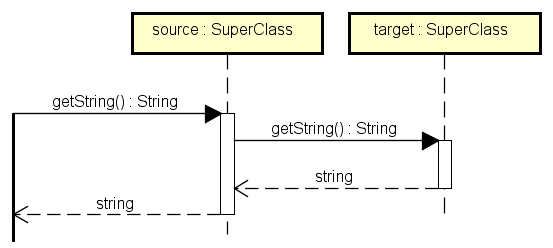
\includegraphics[width=\linewidth]{sd_exact_super}
  \caption{Szenario ExactTypeMatcher}
  \label{abb:sd_exact_super}

\end{minipage}
\end{figure}

\myparagraph{Definition}
\begin{matcherEquivDef}{ExactTypeMatcher}
\matchTyp{A}{exact}{B} \text{ wenn } A = B
\end{matcherEquivDef}
\begin{matcherConvDef}{ExactTypeMatcher}{
Sei $ m $ eine Methode des Typen $ A $ und $ B $.}
\delegate{A.m}{B.m}
\end{matcherConvDef}\\
Ein Beispiel f�r die Verwendung des Matchers ist in \appref{exactMatcherExample} zu finden.
\subsubsection{GenTypeMatcher}\label{genTypeMatcher}
\myparagraph{Szenario}
Dieser Matcher stellt das Matching zwischen zwei Typen her, die in einer Vererbungsbeziehung stehen. Speziell erlaubt dieser Matcher das Matching eines Supertyps als Source-Typen mit einem Subtypen als Target-Typen. In dem Szenario wird neben dem Typ SuperClass aus \abbref{cd_superclass} von einem weiteren Typen SubClass ausgegangen. Dabei stehen diese beiden Typen in einer Vererbungsbeziehnung, die in \abbref{cd_subclass_extends_superclass} dargestellt wird. Der Aufruf einer Methode auf dem Source-Objekt f�hrt zu einer Delgation der Methode an das Target-Objekt (siehe \abbref{sd_gen_super2sub}).
\begin{figure}[H]
\begin{minipage}[b]{.33\linewidth}
  \centering
  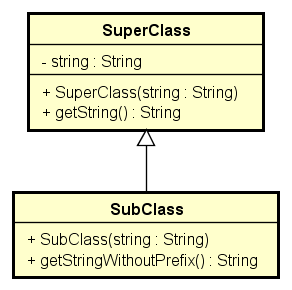
\includegraphics[width=\linewidth]{cd_subclass_extends_superclass}
  \caption{Beziehung zwischen SuperClass und SubClass}
  \label{abb:cd_subclass_extends_superclass}

\end{minipage}%
\hspace{.04\linewidth}% Abstand zwischen Bilder
\begin{minipage}[b]{.63\linewidth}


  \centering
  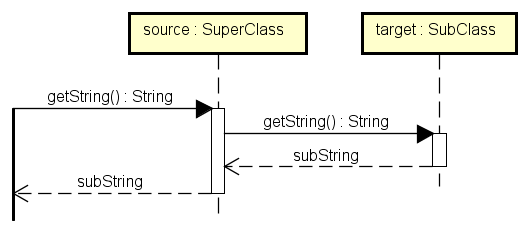
\includegraphics[width=\linewidth]{sd_gen_super2sub}
  \caption{Szenario GenTypeMatcher}
  \label{abb:sd_gen_super2sub}

\end{minipage}
\end{figure}




\myparagraph{Definition}
\begin{matcherEquivDef}{GenTypeMatcher}
\matchTyp{A}{gen}{B} \text{ wenn } \inhTyp{B}{A}
\end{matcherEquivDef}
\begin{matcherConvDef}{GenTypeMatcher}{
Sei $ m $ eine Methode des Typs $ A $, die aufgrund der Vererbung auch von Typ $ B $ bereitgestellt wird.}
\delegate{A.m}{B.m}
\end{matcherConvDef}\\
Ein Beispiel f�r die Verwendung des Matchers ist in \appref{genMatcherExample} zu finden.

\subsubsection{SpecTypeMatcher}\label{specTypeMatcher}
\myparagraph{Szenario}
Analog zum GenTypeMatcher stellt der SpecTypeMatcher ebenfalls das Matching zwischen Typen fest, die in einer Vererbungsbeziehung stehen. Allerdings ist der Source-Typ in diesem Matcher der Subtyp und der Target-Typ der Supertyp. In dem Szenario wird wiederum von den Klassen SuperClass und SubClass aus \abbref{cd_subclass_extends_superclass} ausgegangen. Der Methodenaufruf erfolgt hier aber auf dem Subtypen und wird an den Supertypen delegiert (siehe \abbref{sd_spec_sub2super}).
\myScalableFigure[0.7\linewidth]{sd_spec_sub2super}{Szenario SpecTypeMatcher}{sd_spec_sub2super}
\noindent
Dabei sind zwei Methodenaufrufe auf dem Subtyp beschrieben. W�hrend der Aufruf der Methode getString erfolgreich delegiert werden kann, f�hrt der Aufruf der Methode getStringWithoutPrefix zu einem Laufzeitfehler, da der Matcher keine passende Methode in dem Target-Typ ermitteln kann. Dieses Problem tritt bei allen Methoden auf, die nicht vom Supertyp an den Subtyp vererbt oder �berschrieben wurden.\footnote{Anders gesagt, erm�glicht dieser Matcher einen Downcast, bei dem ein Objekt eines allgemeinen Typen auf einen spezielleren Typen gecastet wird. Das Problem bzgl. des fehlschlagenden Methodenaufrufs in der beschriebene Form ist bei einem Downcast allgegenw�rtig.} Aus diesem Grund muss diese Bedingung in der Definition der Konvertierung dieses Matchers mit aufgenommen werden.
\myparagraph{Definition}
\begin{matcherEquivDef}{SpecTypeMatcher}
\matchTyp{A}{genspec}{B} \text{ wenn } \inhTyp{A}{B}
\end{matcherEquivDef}
\begin{matcherConvDef}{SpecTypeMatcher}{
Sei $ m $ eine Methode des Typs $ A $, die von $ B $ an $ A $ vererbt wurde.}
\delegate{A.m}{B.m}
\end{matcherConvDef}\\
Ein Beispiel f�r die Verwendung des Matchers ist in \appref{specMatcherExample} zu finden.
\subsubsection{WrappedTypeMatcher}\label{wrappedTypeMatcher}
\myparagraph{Szenario}
Die bisherigen Type-Matcher sind in der Lage das Matching f�r zwei Typen festzustellen, ohne daf�r R�cksicht auf deren innere Struktur nehmen zu m�ssen. Dies ist f�r identische oder hierarchisch organisierte Typen auch nicht notwendig. Es ist jedoch auch denkbar, dass sich beiden Typen auf anderem Wegen assoziieren lassen. Ein Beispiel daf�r w�re Boxed- bzw. - noch allgemeiner gefasst - Wrapper-Typen. In \abbref{cd_subclass_subwrapper} sind zwei Klassen dargestellt, die in einer solchen Beziehung zueinander stehen. Bez�glich des Matchings sind auch hier wiederum zwei F�lle zu unterscheiden. Der erste Fall, in dem das Matching des Source-Typen SubClass mit dem Typen eines Attributs wrapped des Traget-Typen SubWrapper festgestellt werden kann, ist in \abbref{sd_wrapped_sub2subwrapped} dargestellt.
\begin{figure}[H]
\begin{minipage}[b]{.33\linewidth}
  \centering
  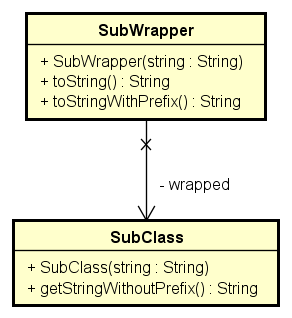
\includegraphics[width=\linewidth]{cd_subclass_subwrapper}
  \caption{Beziehung zwischen SubClass und SubWrapper}
  \label{abb:cd_subclass_subwrapper}

\end{minipage}%
\hspace{.04\linewidth}% Abstand zwischen Bilder
\begin{minipage}[b]{.63\linewidth}


  \centering
  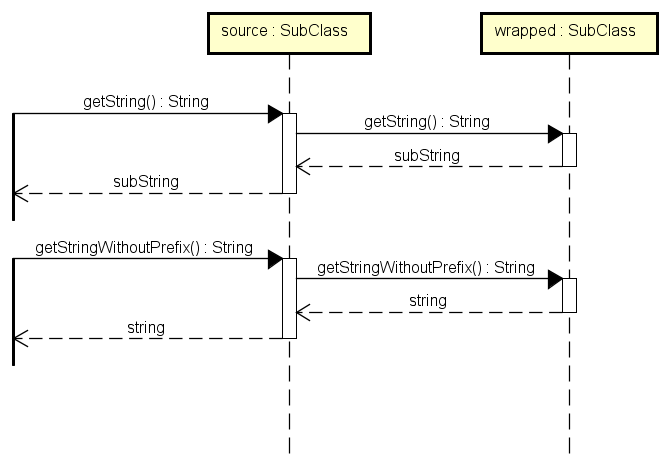
\includegraphics[width=\linewidth]{sd_wrapped_sub2subwrapped}
  \caption{Szenario WrappedTypeMatcher}
  \label{abb:sd_wrapped_sub2subwrapped}

\end{minipage}
\end{figure}
\noindent
Der WrappedTypeMatcher stellt das Matching f�r ein solches Szenario fest. Das Matching der beiden Typen beruht letztendlich auf einem Matching zwischen dem Source-Type und dem Typen eines Attributs des Target-Typs. Der Matcher, �ber den dieses Matching innerhalb des WrappedTypeMatchers festgestellt wird, wird als interner Matcher bezeichnet. In dem Szenario aus \abbref{sd_wrapped_sub2subwrapped} wird als interner Matcher der bereits beschriebene ExactTypeMatcher verwendet, weil der Source-Type und der Typ des Attributs wrapped identisch sind.
\myparagraph{Definition}
\begin{matcherEquivDef}{WrappedTypeMatcher}
\matchTyp{A}{wrapped}{B} \text{ wenn } \exists \selTyp{B}{attr} : \matchTyp{A}{M}{attr}
\end{matcherEquivDef}\\
Der zuvor genannte interne Matcher wird in der Definition mit $M$ beschrieben, was stellvertretend f�r eine Menge von Matchern steht. Als interne Matcher kommen hierbei der ExactTypeMatcher, der GenTypeMatcher und der SpecTypeMatcher in Frage.\\
\begin{matcherConvDef}{WrappedTypeMatcher}{
Sei $m$ eine Methode des Typs $A$. Sei weiterhin $B$ ein Typ, der ein Attribut vom Typ $attr$ enth�lt, f�r den gilt $\matchTyp{A}{M}{attr}$.
}
\delegate{A.m}{(\applyMatcher{A}{attr}).m}
\end{matcherConvDef}\\
Ein Beispiel f�r die Verwendung des Matchers in Bezug auf das o.g. Szenario ist in \appref{wrappedMatcherExample} zu finden. Au�erdem sind dort auch weitere Szenarien aufgef�ht, in denen der GenTypeMatcher oder der SpecTypeMatcher als interner Matcher zur Anwendung kommen.


\subsubsection{WrapperTypeMatcher}\label{wrapperTypeMatcher}
\myparagraph{Szenario}
Dieser Matcher stellt das Pendant zum WrappedTypeMatcher dar. Der Unterschied bzgl. des Szenarios besteht darin, dass nun der Source-Typ derjenige ist, der ein Attribut enth�lt, f�r dessen Typ ein Matching zum Target-Typen �ber den ExactTypeMatcher, den GenTypeMatcher oder den SpecTypeMatcher festgestellt werden kann. F�r das Szenario ist wiederum von den Typen aus \abbref{cd_subclass_subwrapper} auszugehen. Die Delegation der m�glichen Methodenaufrufe am Source-Typen, sind in \abbref{sd_wrapper_subwrapped2sub} abgebildet. Hierbei ist hervorzuheben, dass zur Laufzeit das Objekt vom Target-Typen in das Attribut des Objektes vom Source-Typen injiziert wird. Dies soll in \abbref{sd_wrapper_subwrapped2sub} durch die Bezeichnung des Targets mit wrapped (dem Namen des Attributs) und target dargestellt werden. Eine Methoden-Delegation findet nur dann statt, wenn sie auch im Wrapper-Typen (Source-Typen) implementiert wurde\footnote{Implementierung von SubWrapper: siehe \appref{matcherExamples} \lstref{LST_subwrapper_impl}}.
\myScalableFigure[0.8\linewidth]{sd_wrapper_subwrapped2sub}{Szenario WrapperTypeMatcher}{sd_wrapper_subwrapped2sub}
\myparagraph{Definition}
\begin{matcherEquivDef}{WrapperTypeMatcher}
\matchTyp{A}{wrapper}{B} \text{ wenn } \exists\selTyp{A}{attr} : \matchTyp{B}{M}{attr} 
\end{matcherEquivDef}\\
Wie an dieser Beschreibung zu erkennen ist, werden auch hier wieder ein interner Matcher $M$ verwendet. Analog zum WrappedTypeMatcher kommen auch hier der ExactTypeMatcher, der GenTypeMatcher und der SpecTypeMatcher in Frage.\\
\begin{matcherConvDef}{WrappedTypeMatcher}{
Sei $m$ eine Methode des Typs $A$.
}
\delegate{A.m}{A.m}
\end{matcherConvDef}\\
Ein Beispiel f�r die Verwendung des Matchers in Bezug auf das o.g. Szenario ist in \appref{wrapperMatcherExample} zu finden. Au�erdem sind dort auch weitere Szenarien aufgef�ht, in denen der GenTypeMatcher oder der SpecTypeMatcher als interner Matcher zur Anwendung kommen.

\subsubsection{StructuralTypeMatcher}\label{structTypeMatcher}
Die bisher beschriebene Type-Matcher erlauben lediglich ein Matching zwischen Typen, die syntaktisch miteinander in einer direkten Beziehung stehen. Ein Ziel dieser Arbeit ist es jedoch Typen, die voneinander syntaktisch unabh�ngig sind, miteinander zu matchen, um darauf aufbauend, deren Semantik zu �berpr�fen. Hierf�r soll wie auch in \cite{hummel08} die strukturelle �bereinstimmung der beiden Typen ermittelt und verwendet werden. Diesem Zweck dient der StructuralTypeMatcher.
\myparagraph{Szenario}
Um die grundlegenden Eigenschaften des StructuralTypeMatchers darzustellen, wird von einem Szenario ausgegangen, in dem der Target-Typ (angebotenes Interface) zu jeder Methode des Sources-Typs (ben�tigtes Interface) eine passende Methode anbietet. Eine Kombination von angebotenen Interfaces ist somit in diesem Szenario nicht notwendig.\\\\
\abbref{cd_superrsubp_subrsuperp} zeigt die Typen, von denen in dem folgenden Szenario ausgegangen wird. Hierbei sind zwei Klassen aufgef�hrt, die jeweils zwei Methoden anbieten. Die Parameter- und R�ckgabetypen der Methoden sind aus den Szenarien zu den anderen Matchern bekannt. Die Klasse SuperReturnSubParamClass wird in dem folgenden Szenario als Source-Typ und die Klasse SubReturnSuperWrapperParamClass wird als Target-Typ verwendet. Um die strukturelle �bereinstimmung der beiden Typen festzustellen, muss der StructuralTypeMatcher ein Matching zwischen den Parameter- und R�ckgabetypen der einzelnen Methoden herstellen. Dies erfolgt wiederum �ber interne Type-Matcher. An dieser Stelle k�nnen alle zuvor genannten Type-Matcher als interner Type-Matcher verwendet werden. Die Delegation der Methode-Aufrufe erfolgt dann an die Methode des Target-Objekts, die als �bereinstimmende bzw. passende Methode ermittelt wurde (siehe \abbref{sd_struct}). Da beide Methoden eine unterschiedliche Anzahl von Parametern haben, ist in diesem Beispiel leicht nachzuvollziehen, welche Methoden zusammenpassen. Als interner Type-Matcher wurde in diesem Szenario der GenTypeMatcher verwendet. 
\myBigFigure{cd_superrsubp_subrsuperp}{SuperReturnSubParamClass und SubReturnSuperParamClass}{cd_superrsubp_subrsuperp}
\myBigFigure{sd_struct}{Szenario StructTypeMatcher}{sd_struct}
\myparagraph{Definition}
\begin{matcherEquivDef}{StructuralTypeMatcher}
&\matchTyp{A}{struct}{B} \text{ wenn}\\
&\exists(A.m(MP) : MR) : \exists (B.n(NP):NR):\matchTyp{MP}{P}{NP} \wedge \matchTyp{NR}{R}{MR}
\end{matcherEquivDef}\\
Da die Notation es nicht hergibt, ist zus�tzlich zu erw�hnen, dass die Reihenfolge der Parameter in $m$ und $n$ irrelevant ist.\\
%fuer Formatierung
\\
\begin{matcherConvDef}{StructuralTypeMatcher}{
Sei $m$ eine Methode des Typs $A$.\\
Der R�ckgabetyp von $m$ sei $MR$ und $MP$ der Parametertyp von $m$.\\
Weiterhin sei $n$ eine Methode des Typs $B$.\\
Der R�ckgabetyp von $n$ sei $NR$ und $NP$ der Parametertyp von $n$.
}
\delegate{A.m(MP):MR}{B.n(\applyMatcher{NP}{MP}) : \applyMatcher{MR}{NR}}
\end{matcherConvDef}\\
Ein Beispiel f�r die Verwendung des Matchers in Bezug auf das o.g. Szenario ist in \appref{structMatcherExample} zu finden. Au�erdem sind dort auch weitere Szenarien aufgef�ht, in denen andere Matcher als interner Matcher zur Anwendung kommen.

%\subsubsection{Typ- und Methoden-Konvertierungsvarianten}\label{type_meth_conv}
Die Konvertierung der einzelnen Type-Matcher liefert eine Menge von so genannten Typ-Konvertierungsvarianten. Eine Typ-Konvertierungsvariante beschreibt eine M�glichkeit, wie ein Typ in einen anderen konvertiert werden kann. Zu diesem Zweck enth�lt eine Typ-Konvertierungsvariante zwei Arten von Information: 
\begin{enumerate}
\item Objekterzeugungsrelevante Informationen
\item Methodendelegationsrelevante Informationen
\end{enumerate}
Typ-Konvertierungsvarianten werden von einem konkreten Typ-Matcher f�r jede m�gliche Form der �bereinstimmung erzeugt. Ein Matcher erzeugt, wenn �berhaupt, immer nur eine Typ-Konvertierungsvariante.\\\\
Die objekterzeugungsrelevanten Informationen sorgen daf�r, dass das Proxy-Objekt f�r den Source-Typ korrekt erzeugt werden kann.\\\\
Die methodendelegationsrelevanten Informationen werden verwendet um so genannten Methoden-Konvertierungsvarianten zu erzeugen. Diese sorgen daf�r, dass das R�ckgabe-Objekt und die Parameter-Objekte beim Methodenaufruf korrekt konvertiert werden und dass der Aufruf an die richtige Methode des Target-Typs delegiert wird.\\\\
Speziell der StructuralTypeMatcher erm�glicht es, zu einer Methode des Source-Typen mehrere methodendelegationsrelevanten Informationen zu erhalten. Das liegt daran, dass dieser Matcher alle Methoden des Source- und des Target-Typen miteinander auf �berstimmung �berpr�ft. Dabei kann es vorkommen, dass eine Methode des Source-Typen mit mehreren Methoden des Target-Typen - oder umgekehrt - �bereinstimmt.
In \abbref{konvar_voll} ist dieser Zusammenhang f�r ein angebotenes Interface AIv und einem erwarteten Interface EI, welche jeweils zwei Methoden enthalten (AM * bzw. EM *), skizziert. Hier wird angenommen, dass jede der angebotenen Methoden strukturell mit jeder der erwarteten Methoden �bereinstimmen w�rde. Dementsprechend enth�lt die Typ-Konvertierungsvariante (TKV) methodendelegationsrelevante Informationen, aus denen insgesamt 4 Methoden-Konvertierungsvarianten erzeugt werden, wovon jede eine Konvertierung entlang der eingezeichneten Pfeile erm�glicht.\\\\
Dabei gilt jedoch, aufgrund der �berlegungen zur Kombination von angebotenen Komponenten (siehe auch \abbref{combinated_components}), dass eine Typ-Konvertierungsvariante nicht zu jeder der erwarteten Methoden solche methodendelegationsrelevanten Informationen enth�lt. \abbref{konvar_unv} zeigt einen solchen Fall mit dem angebotenen Interface AIu.
\begin{figure}[H]
\begin{minipage}[b]{.48\linewidth}
  \centering
  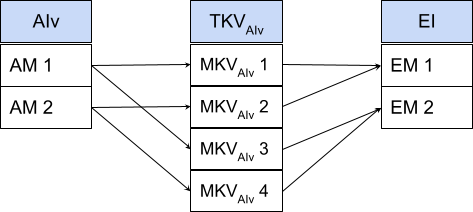
\includegraphics[width=\linewidth]{konvar_voll}
  \caption{Typ- und Methoden-Konvertierungsvarianten von AIv}
  \label{abb:konvar_voll}

\end{minipage}%
\hspace{.04\linewidth}% Abstand zwischen Bilder
\begin{minipage}[b]{.48\linewidth}


  \centering
  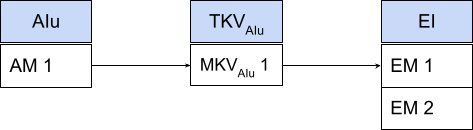
\includegraphics[width=\linewidth]{konvar_unv}
  \caption{Typ- und Methoden-Konvertierungsvarianten von AIu}
  \label{abb:konvar_unv}

\end{minipage}
\end{figure}

